\section{Introduction and background}

TK history of system dynamics models, comparison to PK models, light
discussion of bednets model, and Homie et al's SD model of Hep C.

Wikipedia says: (from \url{http://en.wikipedia.org/wiki/System_dynamics}, accessed 7/21/2011)
\begin{quote}
System dynamics was created during the mid-1950s[3] by Professor Jay
Forrester of the Massachusetts Institute of Technology. In 1956,
Forrester accepted a professorship in the newly-formed MIT Sloan
School of Management. His initial goal was to determine how his
background in science and engineering could be brought to bear, in
some useful way, on the core issues that determine the success or
failure of corporations. Forrester's insights into the common
foundations that underlie engineering, which led to the creation of
system dynamics, were triggered, to a large degree, by his involvement
with managers at General Electric (GE) during the mid-1950s. At that
time, the managers at GE were perplexed because employment at their
appliance plants in Kentucky exhibited a significant three-year
cycle. The business cycle was judged to be an insufficient explanation
for the employment instability. From hand simulations (or
calculations) of the stock-flow-feedback structure of the GE plants,
which included the existing corporate decision-making structure for
hiring and layoffs, Forrester was able to show how the instability in
GE employment was due to the internal structure of the firm and not to
an external force such as the business cycle. These hand simulations
were the beginning of the field of system dynamics.[2]

During the late 1950s and early 1960s, Forrester and a team of
graduate students moved the emerging field of system dynamics from the
hand-simulation stage to the formal computer modeling stage. Richard
Bennett created the first system dynamics computer modeling language
called SIMPLE (Simulation of Industrial Management Problems with Lots
of Equations) in the spring of 1958. In 1959, Phyllis Fox and
Alexander Pugh wrote the first version of DYNAMO (DYNAmic Models), an
improved version of SIMPLE, and the system dynamics language became
the industry standard for over thirty years. Forrester published the
first, and still classic, book in the field titled Industrial Dynamics
in 1961.[2]

From the late 1950s to the late 1960s, system dynamics was applied
almost exclusively to corporate/managerial problems. In 1968, however,
an unexpected occurrence caused the field to broaden beyond corporate
modeling. John Collins, the former mayor of Boston, was appointed a
visiting professor of Urban Affairs at MIT. The result of the
Collins-Forrester collaboration was a book titled Urban Dynamics. The
Urban Dynamics model presented in the book was the first major
non-corporate application of system dynamics.[2]

The second major noncorporate application of system dynamics came
shortly after the first. In 1970, Jay Forrester was invited by the
Club of Rome to a meeting in Bern, Switzerland. The Club of Rome is an
organization devoted to solving what its members describe as the
``predicament of mankind'' -- that is, the global crisis that may
appear sometime in the future, due to the demands being placed on the
Earth's carrying capacity (its sources of renewable and nonrenewable
resources and its sinks for the disposal of pollutants) by the world's
exponentially growing population. At the Bern meeting, Forrester was
asked if system dynamics could be used to address the predicament of
mankind. His answer, of course, was that it could. On the plane back
from the Bern meeting, Forrester created the first draft of a system
dynamics model of the world's socioeconomic system. He called this
model WORLD1. Upon his return to the United States, Forrester refined
WORLD1 in preparation for a visit to MIT by members of the Club of
Rome. Forrester called the refined version of the model
WORLD2. Forrester published WORLD2 in a book titled World Dynamics.[2]

\end{quote}

In parallel to this work, TK David Foster's Mentor at NIH developed
compartmental models for pharmacokinetic data
analysis. Mathematically, these models have precise parallels to the
stock-and-flow models developed by Forrester and colleagues for supply
chain analysis. TK additional paragraphs on this approach, drawing on
books David's friend gave me. The pharmacokinetic applications went
beyond forward simulation to develop methods of statistical inference
for compartmental models. This is a critical development, and one to
which I shall return in the next chapter.

TK connection to the references cited in this NIH RFP for systems modeling
\url{http://grants.nih.gov/grants/guide/pa-files/PAR-08-224.html}
\url{http://ajph.aphapublications.org/cgi/content/full/96/3/452}
\url{http://www.hpsig.com/images/f/f5/SD_background_for_public_health_%284.11.05%29.pdf}
\url{http://www.systemswiki.org/index.php?title=Health_System_Dynamics_References}
\url{http://www.chronicdisease.org/nacdd-initiatives/diabetes/professional-development/act-on-data/SDMResourceList.pdf}

Compartmental modeling has a long tradition in infectious disease
model, as well. TK summary paragraph describing this line of research,
and clearly distinguishing the approach we will take from it. TK
summary of HCV model that explicitly uses systems dynamics approach.

TK review of all pubmed literature that has term system dynamics in
the keywords or something.

TK discussion of bednets model and analogy between this and population
PK approach.

\section{System dynamics model of disease in a population}
At the heart of the new generic disease model is a set of four
compartments representing my fundamental equations of population
health. The compartments represent the population susceptible to the
disease ($S$), the population with the condition ($C$), the population
dead due to other causes ($M$), and the population dead due to the
disease ($D$). The population moves between these boxes following the
arrows shown in the figure, transitioning from $S$ to $C$ with incidence
rate $i$, and from $C$ back to $S$ with remission rate $r$. The susceptible
population transitions into box $M$ with (without-condition) mortality
rate $m$, and the with-condition population transitions into box $M$ with
without-condition mortality rate $m$, and into by $D$ with ``excess
mortality rate'' $f$.

TK parallel between this fundamental model of disease and the demographer's
 basic demographic equation (aka the fundamental balancing equation)
 \url{http://books.google.com/books?id=CR-EXq4y8XAC&lpg=PA5&ots=_jJryixe4z&dq=%22basic%20demographic%20equation%22&pg=PA6#v=onepage&q=%22basic%20demographic%20equation%22&f=false}


\section{Compartmental Model}
\begin{figure}
\begin{center}
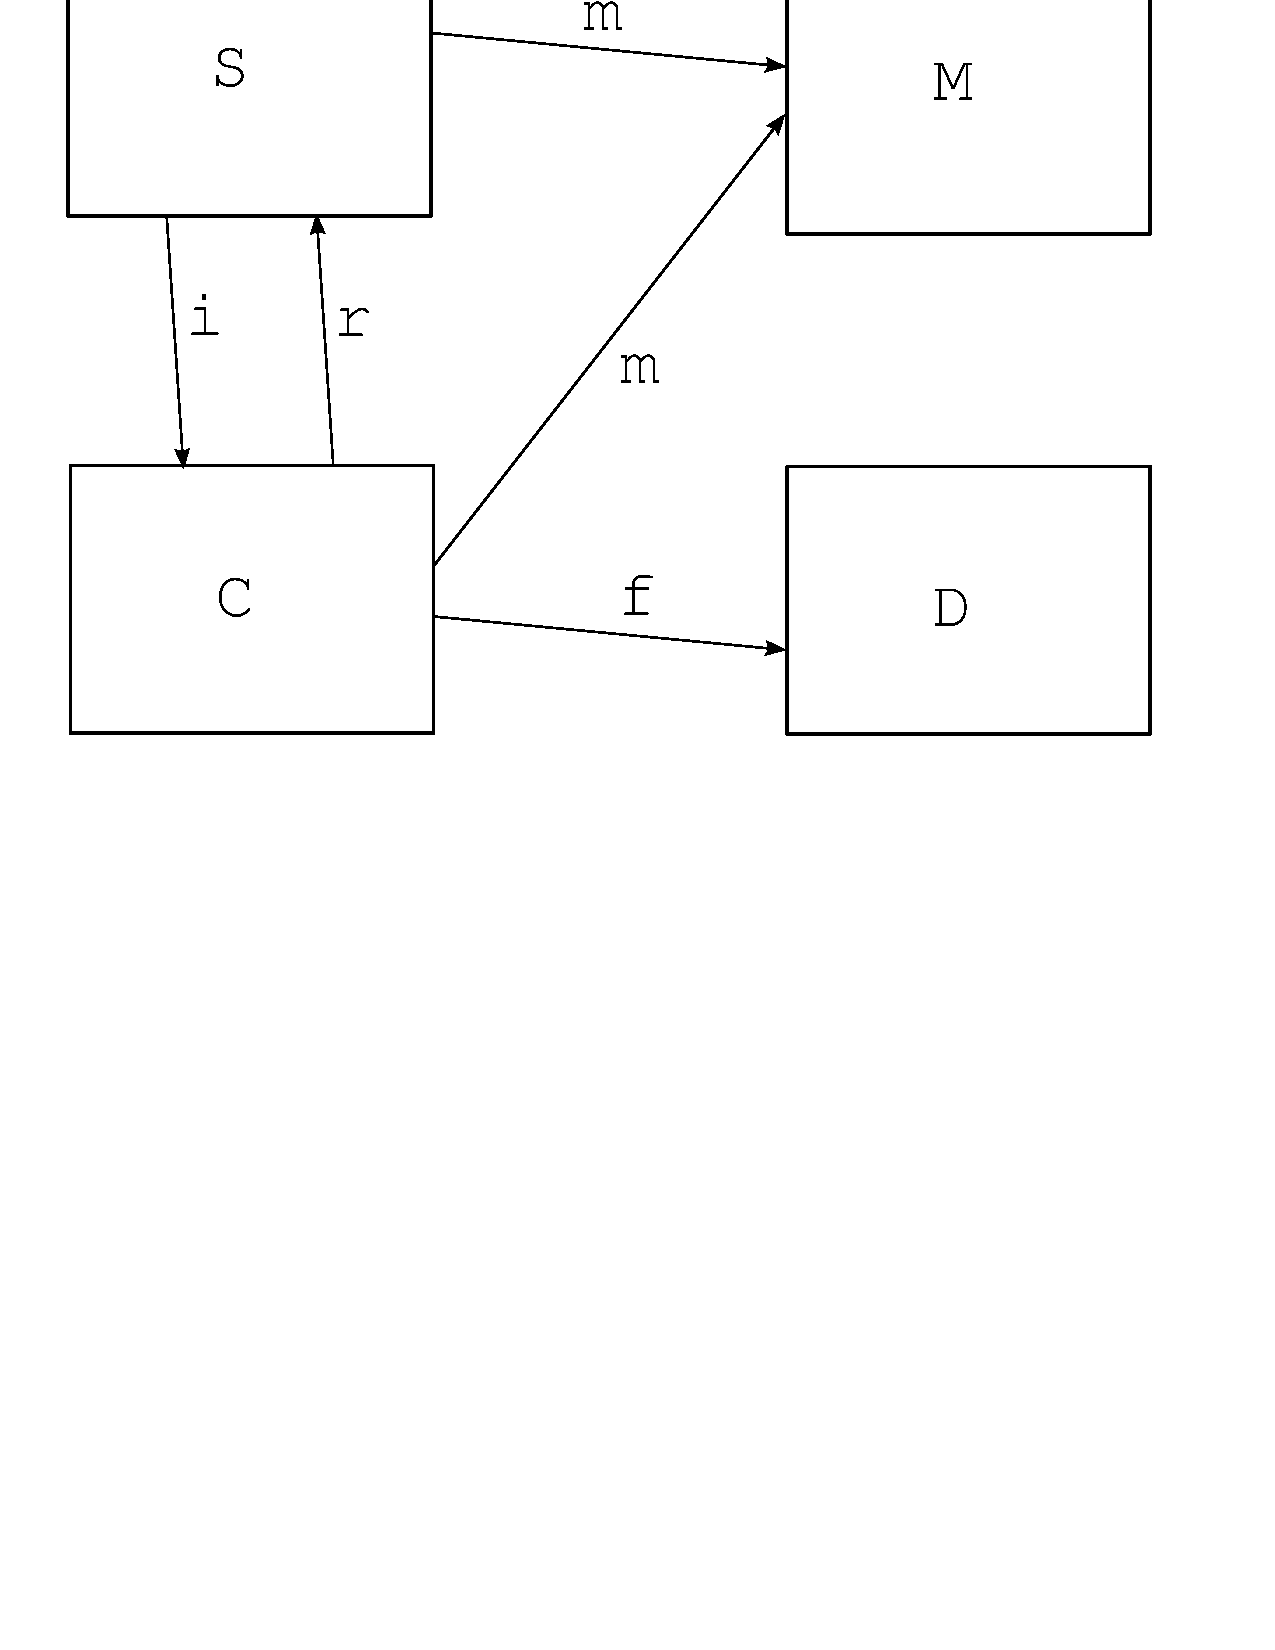
\includegraphics[width=\textwidth]{compartments.pdf}
\end{center}
\caption{TK updated caption; DisMod III uses a 4 compartment model to generate
  age-specific estimates of number without condition ($S$), number
  with condition ($C$), number of deaths not associated with the condition ($M$),
  number of deaths associated with the condition ($D$), incidence rate ($i$),
  remission rate ($r$), without-condition mortality rate ($m$), and
  excess mortality rate ($f$) (all shown in diagram); as well as
  prevalence ($p$), case duration ($X$), relative mortality risk ($RR$), all-cause mortality
  rate ($m_{all}$), and standardized mortality ratio ($SMR$).}
\label{fig:compartmental-model}
\end{figure}

TK Short discussion of what kind of epi study would be designed to
measure each of the important parts of this model. Comment that this
is not always what is available, and the bridge between what we know
and what we want to know will be developed in theory and practice in
several later sections of this book.

Conceptually, it is excess mortality $f$ that has proven hardest to
explain and to understand. This is because in most cases $f$ is a
latent variable, unobservable through most any epi study. Perhaps it
would be clearer to talk about the with-condition mortality rate,
which at least can be measured through a cohort study, and I think
will feel more familiar to the doctor or
epidemiologist. With-condition mortality is $m+f$, and the fact that
$M$ and $D$ are different boxes really is not that important when we
are doing generic disease modeling.

This 4 compartment model is really only a sketch of system dynamics
model I've used however, because it does not show age or time
information. In fact, there are large differences in disease
parameters such as incidence and prevalence as a function of age, and
it is essential for a model to take this into account.  Congenital
abnormalities all have a birth prevalence, while important diseases
such as dementia and Alzheimer's disease have much higher incidence
and prevalence at older ages. Furthermore the incidence and prevalence
of disease, as well as the remission rates and excess-mortality rates
change over time due to shifts in population, changes in prevention or
treatment, or changes in care. And the interdependence between these
factors is complex, but unignorable.  Today's 50-year-olds population
will be tomorrow's 51-year-olds, modulo migration and mortality as
least.

For these reasons, the 4 compartment model is more of a heuristic or
intuitive description of the system dynamics than a precise formal
definition.  A more accurate picture of the system dynamics model
shows the progression of the population as a function of time and age:

TK Time-age expanded version of the compartmental model above.

These figures are not up to the task of giving a full and precise
definition, however, and this is best expressed in terms of a system
of partial differential equations, describing the change in the size
of the compartments as a function of age and time. Although I have
made some simplifying assumptions for practical purposes, I believe
that it is worthwhile to start with the model that I would ideally
like to use, and then simplify it little by little so that it is
appropriately matched to the sparse data and/or the computational
resources available.

TK STOCHASTIC PDE GDM EQUATIONS, an embellishment of the following:

The full model is governed by the following system of partial
differential equations:
\begin{align*}
\frac{\partial S}{\partial (a+t)} &= -(i + m)S + rC,\\
\frac{\partial C}{\partial (a+t)} &= iS - (r + m + f)C,\\
\frac{\partial M}{\partial (a+t)} &= mS + mC,\\
\frac{\partial D}{\partial (a+t)} &= fC,
\end{align*}
where
\begin{align*}
S &= S(a,t) = \text{number without the condition of age $a$ at time $t$}\\
C &= C(a,t) = \text{number with the condition of age $a$ at
  time $t$}\\
M &= M(a,t) = \text{number dead not due to the condition (who would have been) of age $a$ at time
$t$}\\
D &= D(a,t) = \text{number dead due to the condition
  (who would have been) of age $a$ at time $t$}\\[.1in]
i &= i(a,t) = \text{incidence rate for people age $a$ at time $t$}\\
r &= r(a,t) = \text{remission rate for people age $a$ at time $t$}\\
m &= m(a,t) = \text{without-condition mortality rate for people age $a$ at
time $t$}\\
f &= f(a,t) = \text{excess mortality rate for people age $a$ at time
  $t$}
\end{align*}

\subsection{Simplifying assumptions}
\label{theory-forward_sim-compartmental_model-simplying_assumptions}

The first simplification which I have often used is to go from a
stochastic PDE to a deterministic PDE. This was done originally
because of the amount and quality of data available, as well as the
computation speed-up expected.  However, for certain data rich
settings, it may not be desirable. I suspect in the future generic
disease models will want to allow for stochastic PDEs as in the
equations above, and not be tethered by the simplifying assumptions
that I have made here. TK brief discussion of the assumptions inherent
in the deterministic model, and an investigation of how the stochastic
model could deal with these more robustly, for example deviation from
the Markovian assumption that people of age a have the same
with-condition mortality rate, regardless of whether they are a new
case or have had the condition for years. After this simplification,
the system of deterministic PDEs is the following:

\begin{align*}
\frac{\partial S}{\partial (a+t)} &= -(i + m)S + rC,\\
\frac{\partial C}{\partial (a+t)} &= iS - (r + m + f)C,\\
\frac{\partial M}{\partial (a+t)} &= mS + mC,\\
\frac{\partial D}{\partial (a+t)} &= fC,
\end{align*}

The second simplification comes from an assumption that the disease
parameters are not changing substantially with respect to time. TK
implications of simplifying assumptions on time stationarity, and
reduced equation that takes these assumptions into account.  DisMod
III follows the approach used previously, and assumes that the disease
parameters are not changing with time (i.e. the diseases is in endemic
equilibrium),
\[
\frac{\partial S}{\partial t}
=
\frac{\partial C}{\partial t}
=
\frac{\partial D}{\partial t}
=
\frac{\partial M}{\partial t}
=
\frac{\partial i}{\partial t}
=
\frac{\partial r}{\partial t}
=
\frac{\partial m}{\partial t}
=
\frac{\partial f}{\partial t}
=
0.
\]

This assumption on time derivatives is a big one, and deserves careful
assessment. In DisMod II, the default model also included the
assumption that the disease parameters did not change over time, but
an option allowed the model to incorporate assumptions of certain time
trends as well. I will return to the effects of this assumption in
section TK.

The next simplification is on the structure of the rates that dictate
the transitions between compartments (now as a function only of age).
By assuming that these rates are piecewise constant functions of age,
the system of partial differential equations has an explicit solution
for each interval on which the age is constant.

TK rewrite this lead in: Furthermore, DisMod III assumes that the rates are piecewise constant
functions of age, changing rate value only on a specified age mesh.  If
the age mesh is $\{a_0, a_1, \ldots, a_A\}$, then for any $a$ and $a'$
with $a_i \leq a, a' < a_{i+1}$,
\begin{align*}
i(a,t) &= i(a) = i(a')\\
r(a,t) &= r(a) = r(a')\\
m(a,t) &= m(a) = m(a')\\
f(a,t) &= f(a) = f(a')\\
\end{align*}

This permits me to solve the system of equations iteratively, starting
from the first interval, and proceeding interval by interval across
the entire age range. The solution for each age interval, after
assuming that TK FORMAL EQUATOIN OF ASSUMPTION takes the form of a
matrix exponential TK DISPLAY EQUATION.

These assumptions permit DisMod III to solve  explicitly for $S, C, D$
and $M$ iteratively.  The solution is conveniently expressed using the
matrix exponential:
\begin{equation}
\label{eq:ode-soln}
\begin{bmatrix}
S(a_{i+1})\\C(a_{i+1})\\M(a_{i+1})\\D(a_{i+1})
\end{bmatrix}
=
\exp\left(\begin{bmatrix}
-i(a_i)-m(a_i) & r(a_i)             & 0&0 \\
i(a_i)      & -r(a_i) -m(a_i) - f(a_i) & 0&0\\
m(a_i)      & m(a_i)             & 0&0 \\
0        & f(a_i)            & 0&0
\end{bmatrix}
(a_{i+1}-a_i)\right)
\begin{bmatrix}
S(a_i)\\C(a_i)\\M(a_i)\\D(a_i)
\end{bmatrix}
\end{equation}

There is another, related, simplification that is really more a matter
of computational convenience than mathematical simplification.  The
iterative solution to the difference equations above provides the
exact values on an age mesh $\{a_0, a_1, \ldots, a_I\}$, and this
appears in the inner-most loop of the computation, so it is a
significant time saving approximation to use linear interpolation to
fill in prevalence values between the points on the age mesh, instead
of using a more sophisticated differential equation solver to provides
a more precise solution to the system of ODEs. The effects of this
approximation can be minimized by choosing an age mesh appropriately,
and will be examined in more detail qualitatively later in the section
and quantatively in the Chapter TK on numerical algorithms.

Although the primary use of this model is for inference of model
parameters (sometimes called the ``inverse problem''), I can easily
apply it ``forwards'' to show how rates on incidence, remission, and
excess-mortality produce different prevalence curves. The next section
explores this forward simulation through a series of detailed
examples, to build up the reader's intuition around how consistency
forces interrelationships between prevalence, incidence, remission,
and mortality.


\section{Forward simulation examples}

When a generic disease model is initialized with all-cause mortality
data and nothing else, the initial values produce the following set of
consistent age patterns:

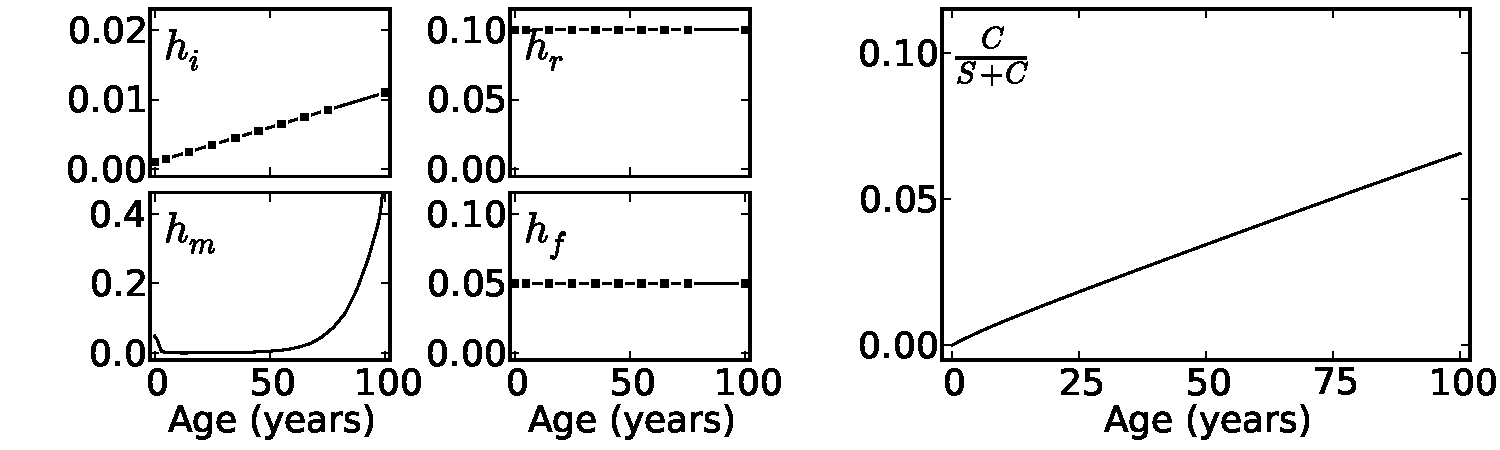
\includegraphics[width=\textwidth]{initial.png}

The next example shows that increasing the remission rate with
incidence and excess mortality unchanged (and all-cause mortality
unchanged as well) leads to a very different age pattern for
prevalence. It is also worth pointing out that since prevalence has
changed with excess mortality and all-cause mortality rates held
constant, the with-condition and background mortality rates have also
changed to maintain consistency.

\includegraphics[width=\textwidth]{more-remission.png}

By changing the incidence rate age pattern to be increasing as a
function of the square root age, I can demonstrate that very similar
prevalence rates are consistent with very different incidence and
remission rates.

\includegraphics[width=\textwidth]{increasing-incidence.png}

Although the prevalence age pattern is largely determined by the
remission, incidence, and mortality rates, the birth prevalence can
also change the shape dramatically.  Here are the results of the same
remission, incidence, and mortality rates as above, but with a birth
prevalence of 20\%.

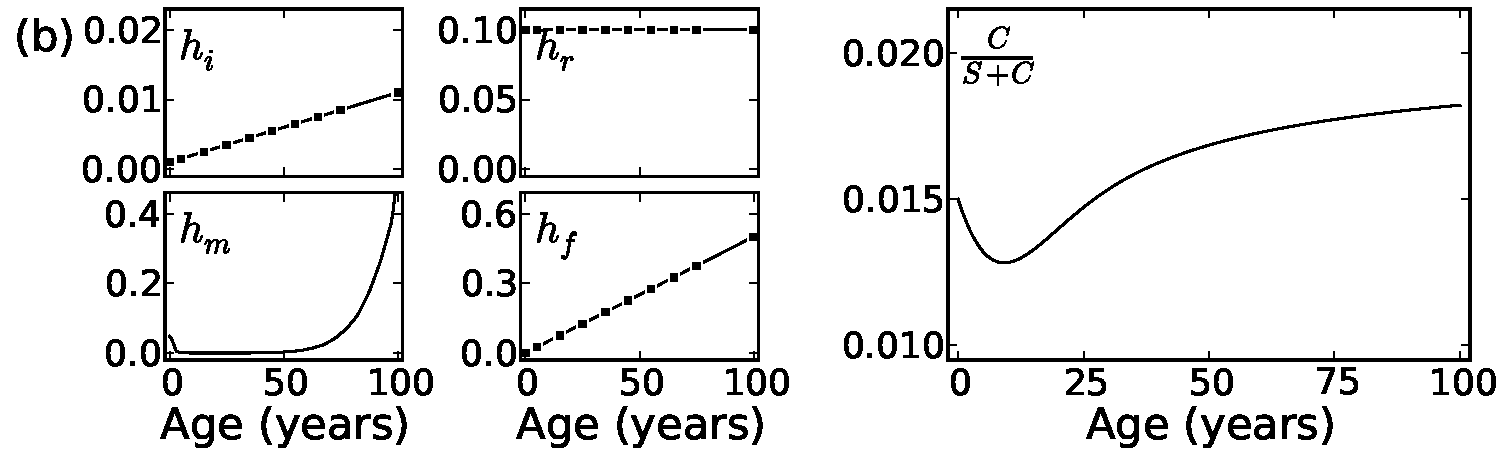
\includegraphics[width=\textwidth]{birth-prevalence.png}

An interesting, and perhaps unexpected feature of this set of
consistent rates above is that when prevalence levels start so high,
the levels remain high during the teenage years, where all-cause
mortality rates are quite low in this population (following the rates
for males in the North American High Income region in 2005), which
produces very low levels of background mortality for these age
groups. In other words, in order for the model to be consistent, it is
necessary to assume that the vast preponderance of teenage deaths are
due to this disease.

Finally, the excess mortality rate (which is the most difficult of the
rates to conceptualize, due to its unobservability) has an effect of
modulating the prevalence that is similar to the remission rate,
although not identical.  The final figure in this series shows the
results of choosing an excess mortality rate to have an age function
equal to ten times the all-cause mortality rate (which is to say a
standardized mortality rate of constant value eleven for all ages).

\includegraphics[width=\textwidth]{higher-smr.png}

The decreasing prevalence after age 65 is worthy of remarking
on. Although the incidence rate is increasing and the remission rate
remains unchanged, having a constant (albeit high) standardized
mortality ratio means that when all-cause mortality rises, the
with-condition mortality rises differentially with such magnitude that
the prevalence of the condition in older populations goes down.

To summarize, this series of figures has shown the intuitive and
less-than-intuitive way that the levels and age patterns of different
epidemiological parameters must be interrelated to satisfy the
fundamental equations of population health (when disease rates for
each age are changing negligibly slowly as a function of time).

The next series of figures continues to build familiarity with the
features of consistent disease modeling, by selecting age patterns for
certain rates based on toy models of a variety of diseases.  For
example, for a disorder like depression, for which there is primarily
incidence in early adulthood, high remission rate, and low excess
mortality, the consistency conditions produce a prevalence age pettern
that peaks at age 25: 

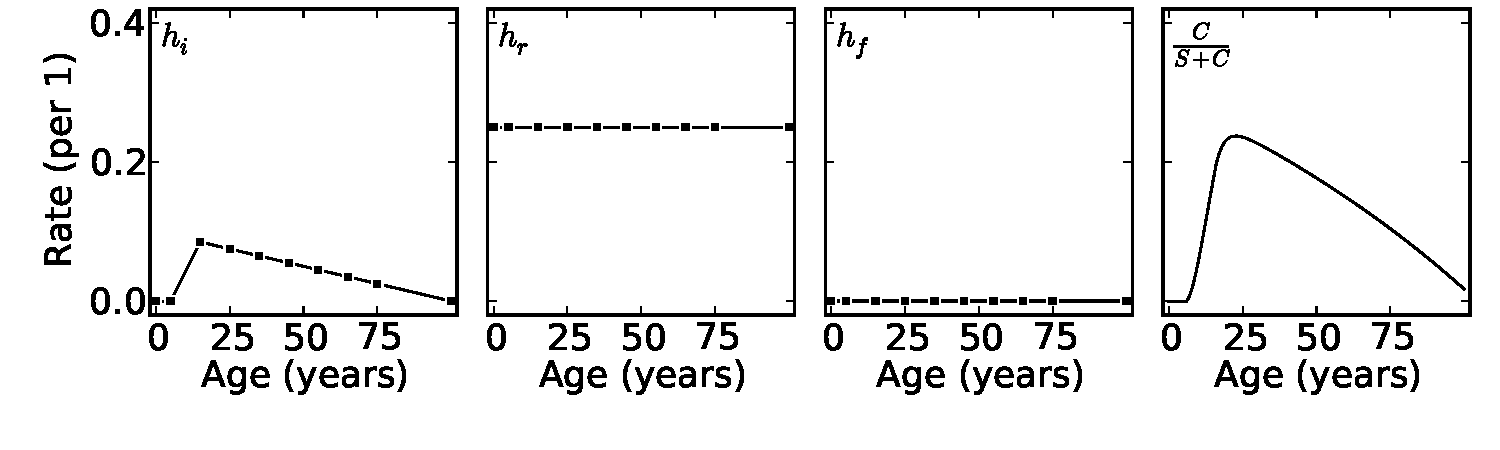
\includegraphics[width=\textwidth]{forward-sim-mental.png}

For a congenital disorder, like TK, with birth prevalence, no
incidence after birth, no remission, and substantial mortality, the
consistent prevalence age pattern is the following:

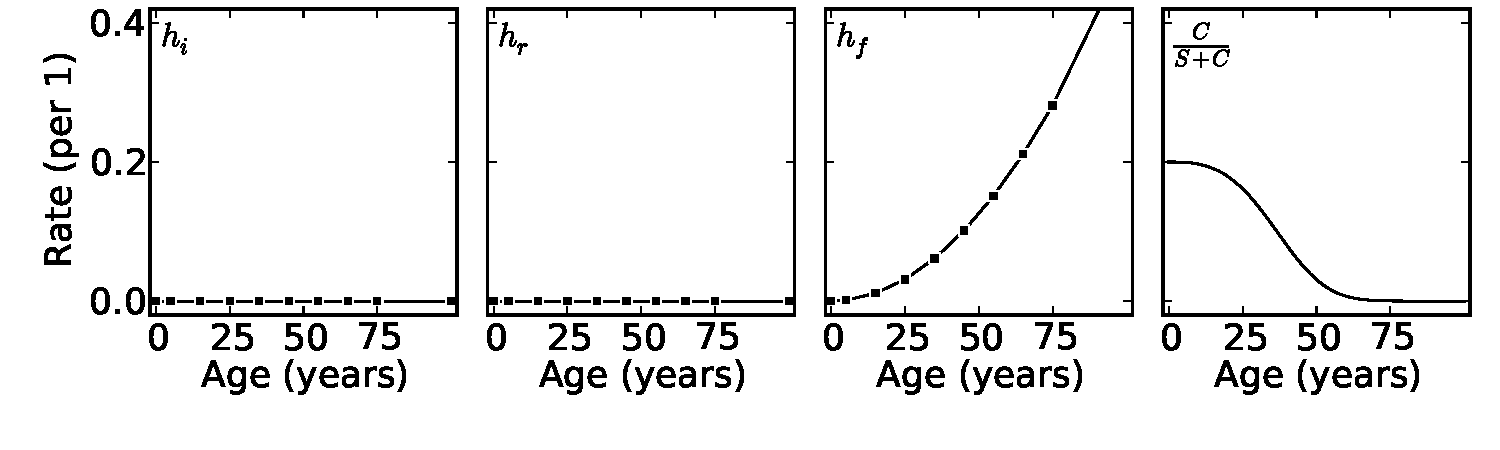
\includegraphics[width=\textwidth]{forward-sim-congenital.png}

For a disorder that affects the elderly, like TK, the consistent age
patterns for mortality, incidence, remission, and prevalence could
look like the following: 

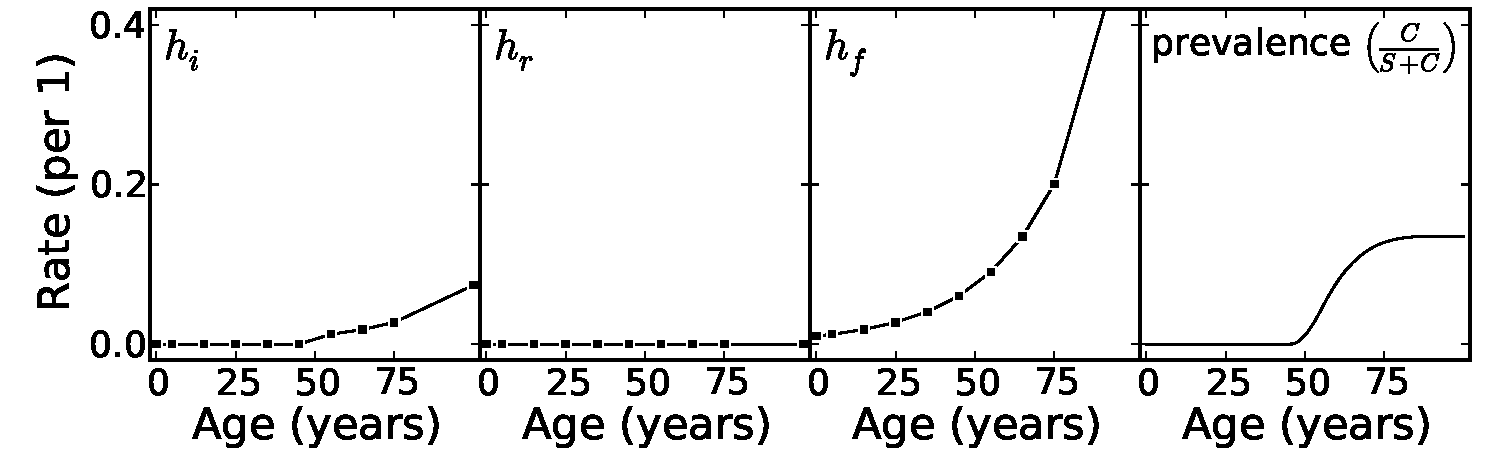
\includegraphics[width=\textwidth]{forward-sim-old_age.png}

And for a disorder related to the reproductive system, like TK, with
substantial excess mortality and incidence during ages 15-60, and
remission that increases substantially at age 55, the consistent age
patterns could look like the following: 

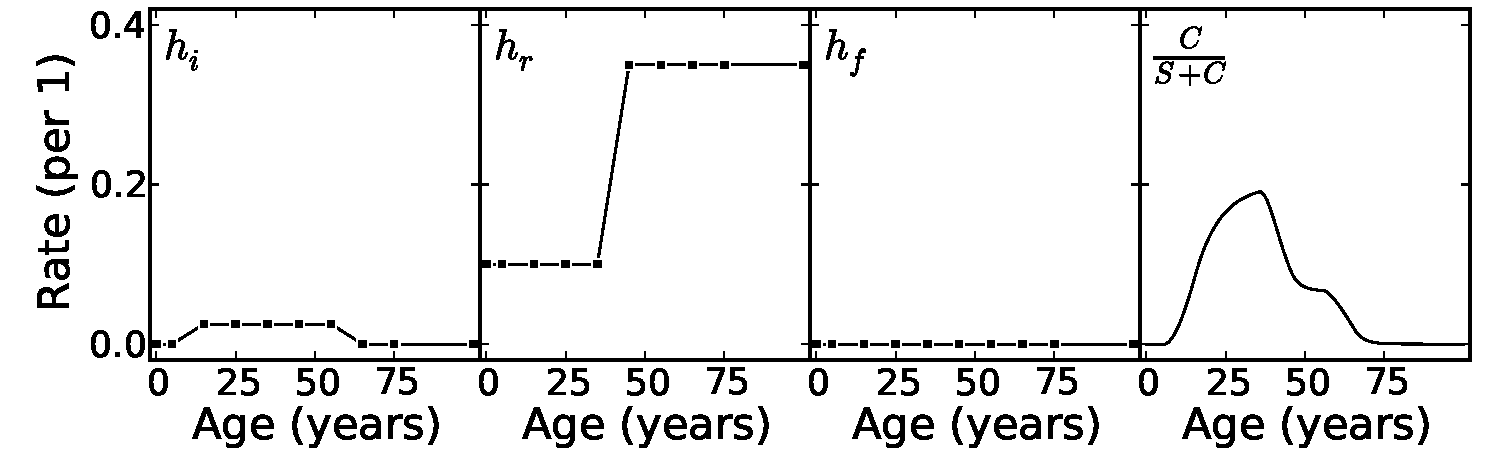
\includegraphics[width=\textwidth]{forward-sim-reproductive.png}

To conclude this series of plots, I've included an "incidence impulse
response" example, showing the prevalence produced to be consistent
with an incidence pattern that is only nonzero for a single age group:

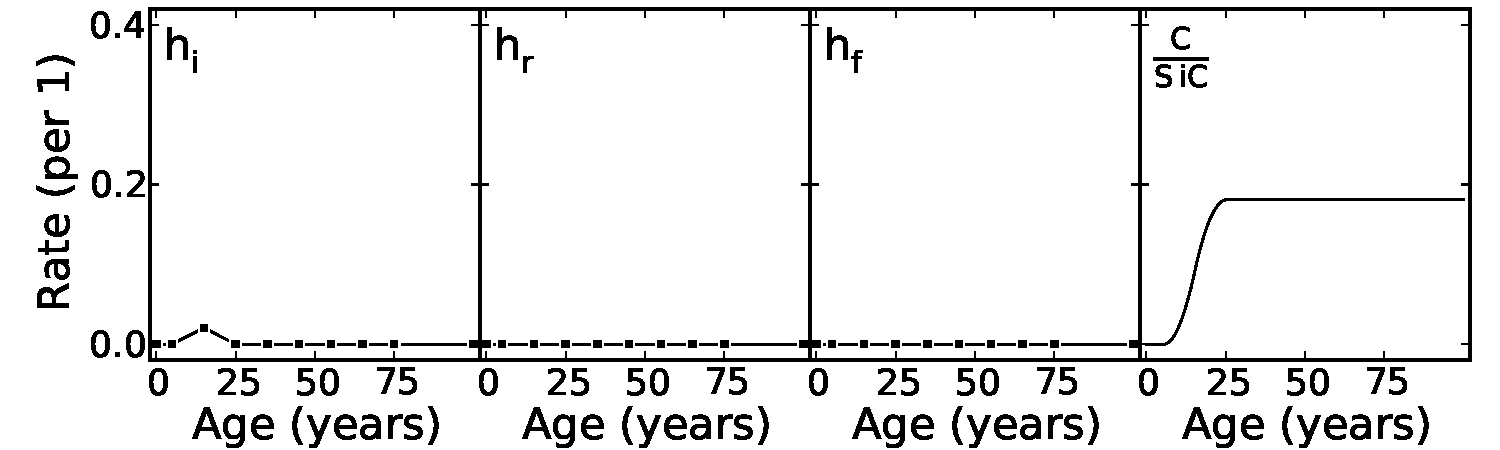
\includegraphics[width=\textwidth]{forward-sim-incidence_pulse.png}

This also provides a mechanism to investigate how wrong the estimates
may become when the assumption that rates are constant over time (for
a given age) is violated. This is the core of my simulation approach
to model validation, to which I will return in section TK.

TK The simulation study approach can be described in full detail here
as well, and can serve as justification for decisions described in the
next two chapters.

\section{What happens to prevalence when the disease incidence or remission or mortality is not constant over time?}

Certain important diseases such as diabetes are widely believed to
have substantial changes in incidence, remission, and mortality rates
over time.  What is the effect of the endemic equilibrium assumption
of the age-specific prevalence. TK plots comparing prevalence from a
synthetic cohort model to a period model using simulation data.
